\documentclass[12pt]{article}

\usepackage{sbc-template}

\usepackage{graphicx,url}
\usepackage[brazil]{babel}
\usepackage[utf8]{inputenc}
\usepackage[T1]{fontenc}
\usepackage[hidelinks]{hyperref}
\usepackage{booktabs}
\usepackage{subfigure}


\sloppy

\title{Smartphone-Based Recognition of Human Activities and Postural Transitions}

\author{Bruno M. Dobrovolski\inst{1}, Eduardo A. Schmoller\inst{1}}

\address{Departamento Acadêmico de Informática -- Universidade Tecnológica Federal do Paraná\\
	Pato Branco -- PR -- Brasil	
	\email{\{brunod,schmoller\}@alunos.utfpr.edu.br}
}

\begin{document} 

\maketitle

%\begin{abstract}
%  This meta-paper describes the style to be used in articles and short papers
%  for SBC conferences. For papers in English, you should add just an abstract
%  while for the papers in Portuguese, we also ask for an abstract in
%  Portuguese (``resumo''). In both cases, abstracts should not have more than
%  10 lines and must be in the first page of the paper.
%\end{abstract}
%
%\begin{resumo}
%  Este meta-artigo descreve o estilo a ser usado na confecção de artigos e
%  resumos de artigos para publicação nos anais das conferências organizadas
%  pela SBC. É solicitada a escrita de resumo e abstract apenas para os artigos
%  escritos em português. Artigos em inglês deverão apresentar apenas abstract.
%  Nos dois casos, o autor deve tomar cuidado para que o resumo (e o abstract)
%  não ultrapassem 10 linhas cada, sendo que ambos devem estar na primeira
%  página do artigo.
%\end{resumo}

\section{Introdução}

%	Exemplo artigo: \url{https://www.elen.ucl.ac.be/Proceedings/esann/esannpdf/es2013-11.pdf}\\

	Este trabalho apresentará resultados da aplicação de métodos de aprendizado de máquinas na predição de movimentos humanos. Foram implementados os seguintes métodos de aprendizado: KNN, Perceptron e SVM. 
	
	Os dados para base para treinamento e teste foram obtidos de \cite{Dua:2017}. Essas informações são referente a sensores de um dispositivo móvel Galaxy Samsung S2. O \textit{smartphone} foi mantido junto ao corpo dos voluntários em atividades de: Levantar, sentar, deitar, caminhar, subir escadas e descer escadas. Os testes foram executados com 30 voluntários e os dados coletados através dos sensores do smartphone, acelerômetro de 3 eixos e giroscópio de 3 eixos.
	
	Os dados obtidos dos sensores foram pré-processados com a aplicação de filtros para remoção de ruídos, amostrados em intervalos constantes de tempo e normalizados. Também foram segmentados separando cada um dos 3 eixos e calculando várias informações estatísicas (totalmente descritas em cite{Dua:2017}), como média, desvio padrão, máximo, mínimo, entre outras, totalizando 561 características.Cada conjunto de dados que representa os movimentos recebeu uma identificação. O conjunto de características e de idenficações (\emph{label}) são entradas para os algoritmos de classificação.
	
	Como forma de validação do processo de aprendizado, o conjunto de dados de entrada foi dividido em dois subconjuntos denominados conjunto de treino e conjunto de testes. O conjunto de treino é utilizado no processo de treinamento, após o processo de treinamento o conjunto de testes é classificado e os resultados são comparados com as resultados esperados.
	
	Ainda, os algorítimos foram alterados através da redução de dimensionalidade com o uso do método PCA. Como esse método não entrega um resultado ótimo, foi necessário variar o número de componentes para encontrar a melhor combinação.

	Como métrica para a determinação da qualidade do processo de aprendizados foram utilizadas a acurácia da predição e utilização do \emph{kappa score}. O \textit{kappa score} funciona como uma validação do resultado apresentado pela acurácia, visto que ele considera em seu calculo os resultados falso-positivos e falso-negativos, colocando peso em cada uma das características. 

\section{Revisão}

	Esta seção apresenta os métodos aplicados para a classificação dos movimentos.

\subsection{Perceptron}

	Separador linear através de uma função de \emph{threshhold}, reta esta que é definida através de pesos. O treinamento de um perceptron consiste na entrada de um conjunto de casos e calcular a saída para cada caso, após cada entrada os pesos são ajustados de forma a minimizar o erro na saída, o erro é definido como a diferença entre a saída e a saída esperada, não existe erro caso a saída e a saída esperada sejam iguais.
	
	Perceptron de uma única camada apenas separam problemas lineares, para a classificação de classes que não sejam separáveis linearmente é necessário um perceptron de múltiplas camadas.
	
\subsection{KNN}

	KNN algoritmo simples que realiza o aprendizado de todas as entradas e classifica as novas entradas com base na similaridade dos casos já aprendidos. Ao realizar a classificação de uma nova entrada é retornado \emph{k} vizinhos mais próximos, classificação se dá pela maioria dos vizinhos.
	
\subsection{SVM}

	SVM é um classificador definindo a separação entre as classes através de um hiperplano, a entrada são dados com \emph{labels} e a saída é um hiperplano ótimo para categorização de novas entradas. Em duas dimensões o hiperplano é representado através de uma reta que divide o plano em duas partes.
	
\subsection{PCA}

	Redutor de dimensionalidade selecionando as principais componentes, entre as formas de encontrar as componentes principais é buscar as projeções que maximizem a variança.
	
\subsection{Testes Estatísticos}

	Testes estatísticos são utilizados para validação de hipóteses usando dados amostrais para decidir sobre a validade da hipótese.
	
	Cenários típicos de uso de testes estatísticos em métodos de aprendizado: adição de etapas de processamento, comparar diversos algoritmos, validação de capacidade de generalização de um classificador. O principio básico é a formulação de hipóteses e decidir se os dados mostram alguma evidencia para rejeição da hipótese.

	\subsubsection{Validação Cruzada}
		
		Validação cruzada é uma técnica que consiste em reservar uma parte do conjunto de dados para serem utilizados para testes após a etapa de treinamento.
		
		Exemplos de métodos para validação cruzada: \emph{HoldOut} (dividir em treino e teste), \emph{K-fold} (k sub conjuntos de treino e teste), \emph{Stratified K-Fold} (cada conjunto contem aproximadamente a mesma porcentagem de amostras de cada classe que o conjunto completo), \emph{Leave-P-Out} (em um conjunto de n casos então n-p serão utilizados para treino e p casos para teste).
		
	\subsubsection{Matriz de Confusão}
	
		Matriz de confusão contem informações sobre o estado real e o estado previsto por um classificador, a performance do sistema é avaliado usando os dados da matriz, em um sistema com duas classes os valores que podem ser calculados são: acurácia (proporção de predições corretas), recall (proporção de casos positivos classificados corretamente), falsos positivos (proporção de casos negativos classificados incorretamente), negativos (proporção de negativos classificados corretamente), falsos negativos (proporção de positivos classificados incorretamente), precisão (proporção de casos positivos classificados corretamente).
		
	\subsubsection{Kappa Score}
	
	Kappa Score mede a confiabilidade de uma classificação entre múltiplos classificadores para um mesmo conjunto de dados, mede a porcentagem de valores de dados na diagonal principal da tabela e, em seguida, ajusta esses valores para a quantidade de concordância que poderia ser esperada em uma classificação aleatória.
	
	Possivel interpretação do resultado do Kappa Score:
	
	Pouca concordância = Menor que 0.20
	
	Razoável concordância = 0.20 até 0.40
	
	Moderada Concordância = 0.40 até 0.60
	
	Boa concordância = 0.60 até 0.80
	
	Concordância muito boa = 0.80 até 1.00	
		
\section{Resultados}
	Com a aplicação dos métodos citados anteriormente foi possível apresentar a Figura \ref{fig:todos}. Esse gráfico representa a busca pelo melhor agrupamento de características utilizando PCA. Como é possível observar, cada um dos métodos tem um comportamento diferente. O Perceptron tem melhores resultados quanto maior for a quantidade de características; Já o KNN não apresenta muitas melhoras; Por fim o SVM tem uma redução da acurácia para maior quantidade de características. É importante notar que apesar da variação nos resultados, as perdas são relativamente pequenas, cerca de 5\%. O código executado partiu de 10 grupos a 260 grupos, com incremento de 10
	\begin{figure}[!htb]
	\centering
	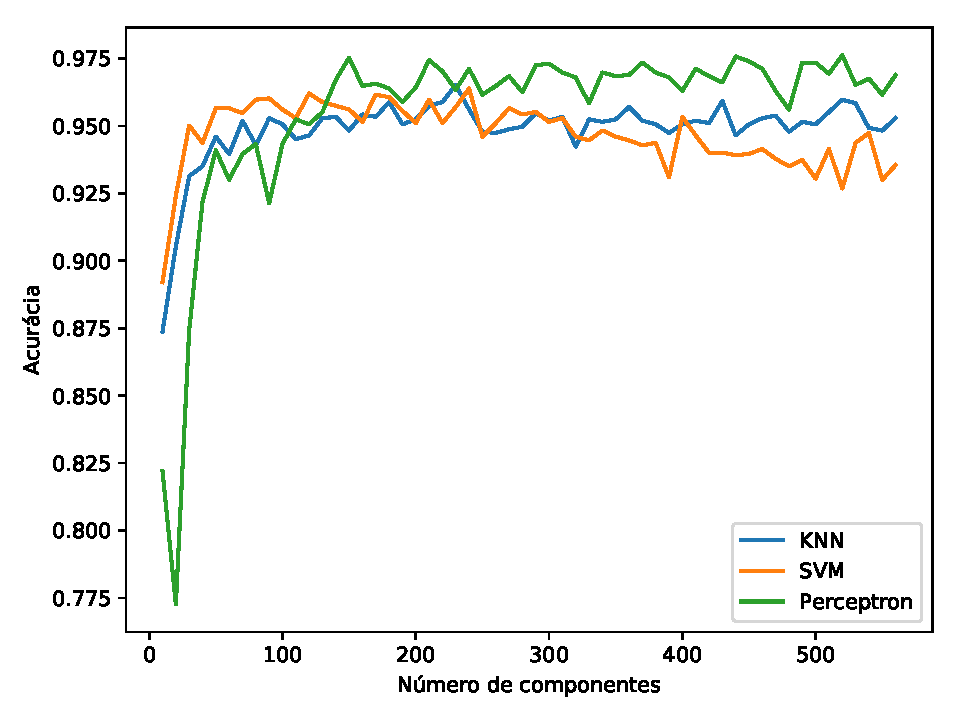
\includegraphics[width=.5\textwidth]{Todos.pdf}
	\caption{Acurácia - KNN, SVM, Perceptron}
	\label{fig:todos}
	\end{figure}
	Porém, é sabido que os bons resultados da acurácia podem não ser reais. Para isso, foi aplicado o Kappa-Score, como explicado anteriormente ele pondera os falso-positivos e falso-negativos, quando comparado à acurácia a diferença entre esses dois valores informa a qualidade do método. A Figura \ref{fig:kappa_accu}, aprenseta essa comparação em relação aos 3 métodos.

	\begin{figure}[h]
	\centering
<<<<<<< HEAD
	\subfigure[Comparação - KNN]{
	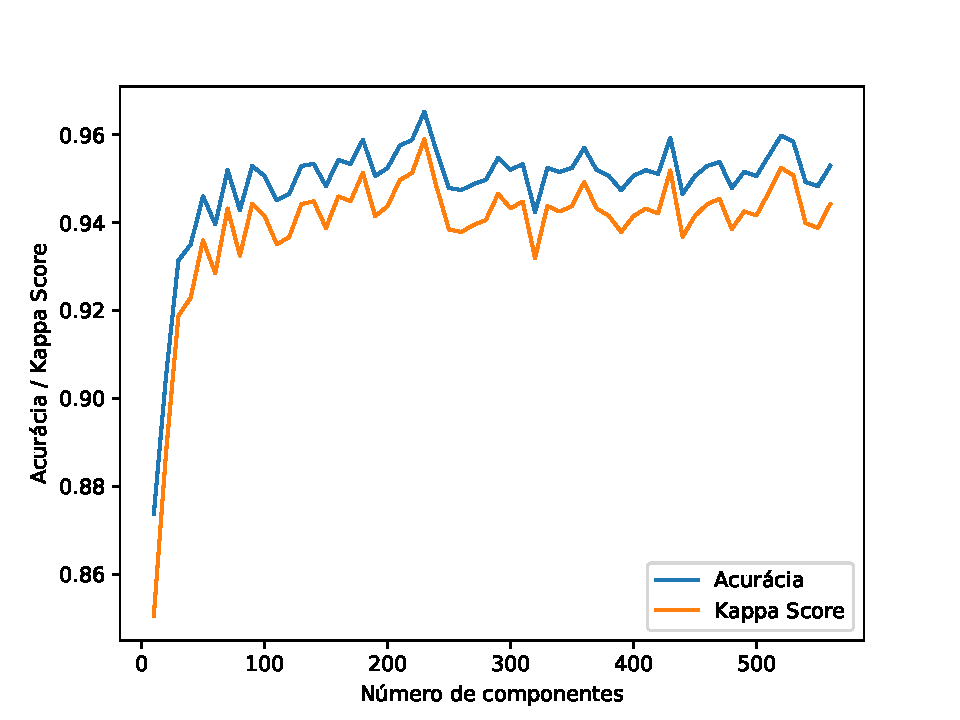
\includegraphics[scale=0.45]{knn_kappa_accu.pdf}}
	\subfigure[Comparação - SVM]{
	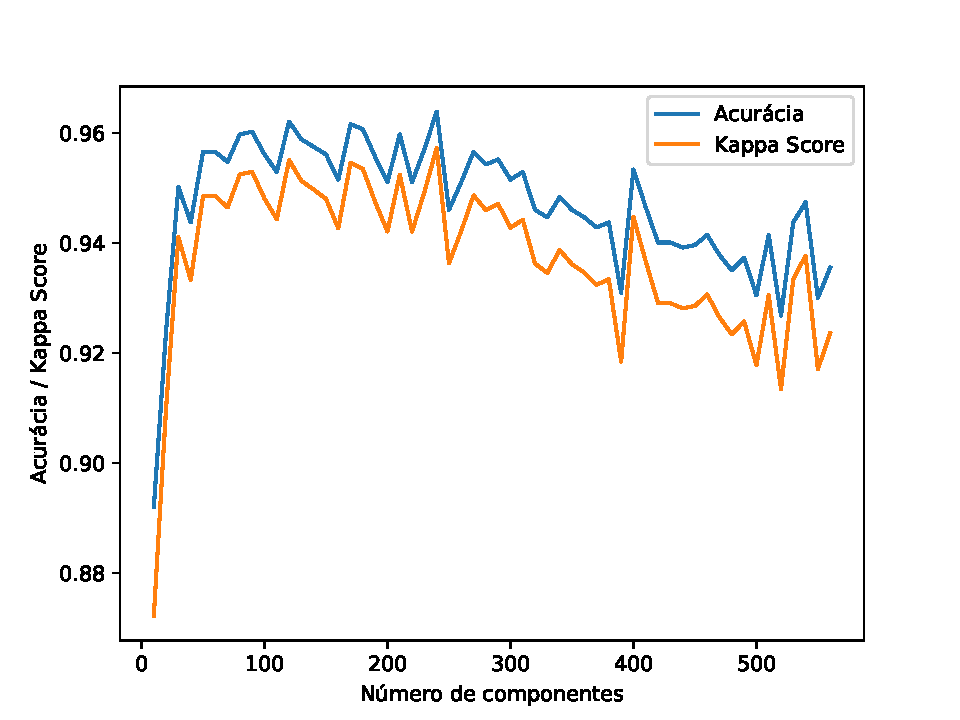
\includegraphics[scale=0.45]{svm_kappa_accu.pdf}}
	\subfigure[Comparação - Perceptron]{
	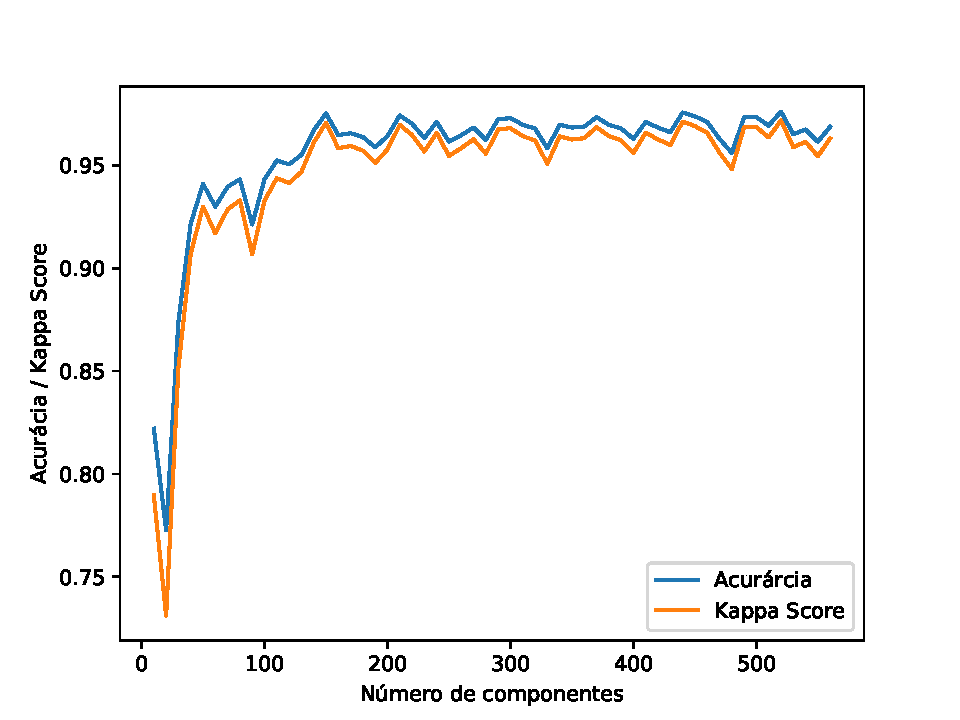
\includegraphics[scale=0.45]{perceptron_kappa_accu.pdf}}
	\caption{Comparação entre Acurácia e Kappa Score }
	\label{fig:kappa_accu}
	\end{figure}
\newpage
	Obervando esses resultados, foi possível obter o melhor agrupamento para cada um dos métodos, essa escolha é apresentada na Tabela \ref{table:resultados}. 
	
	\begin{table}[ht]
		\centering
		\caption{Resultados}
		\label{table:resultados}
		\smallskip
		\begin{tabular}{|l|c|c|c|}
			\hline
			Método& Acurácia & Kappa Score& Agrupamento\\[0.5ex]
			\hline
			&&\\[-2ex]
			KNN &0.9652 & 0.9589 &230\\[0.5ex]
			\hline
			&&\\[-2ex]
			Perceptron &0.9762 &0.9718 &520\\[0.5ex]
			\hline	
			&&\\[-2ex]
			SVM & 0.9663 &0.9572& 240\\[0.5ex]
			\hline
		\end{tabular}
	\end{table}
	
	
	Para o caso ótimo desses conjuntos foi construída a matriz de confusão, afim de validar as informações apresentadas pela acurácia e Kappa Score. As matrizes apresentadas na Figura \ref{fig:confusao}
	
	\begin{figure}[!htb]
	\centering
	\subfigure[Matriz de Confusão - KNN]{
		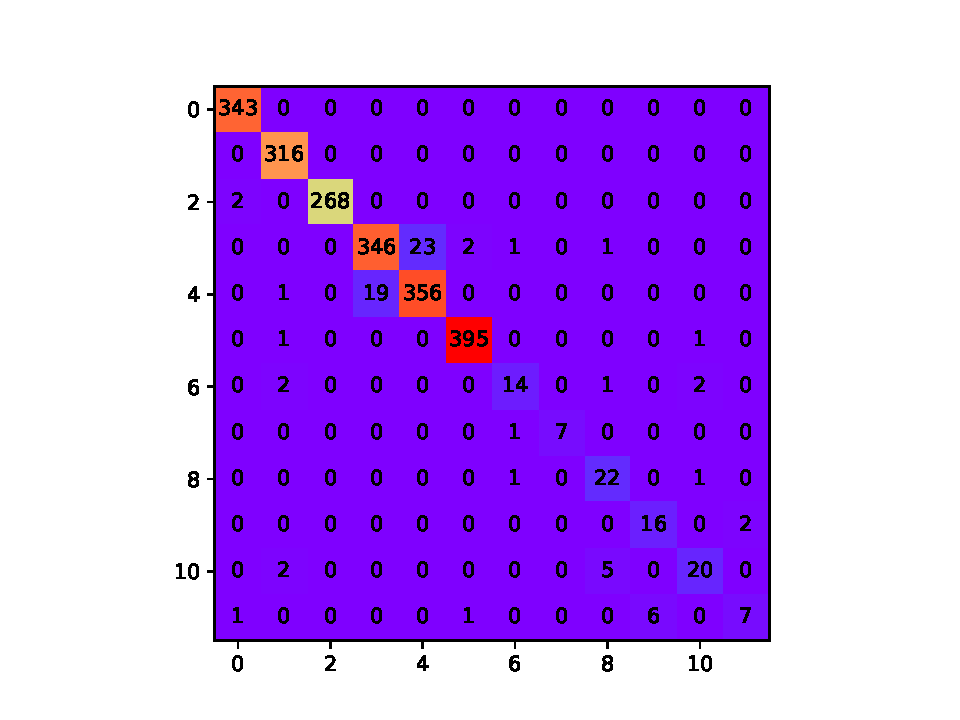
\includegraphics[scale=0.45]{matrix_knn.pdf}}
	\subfigure[Matriz de Confusão - SVM]{
		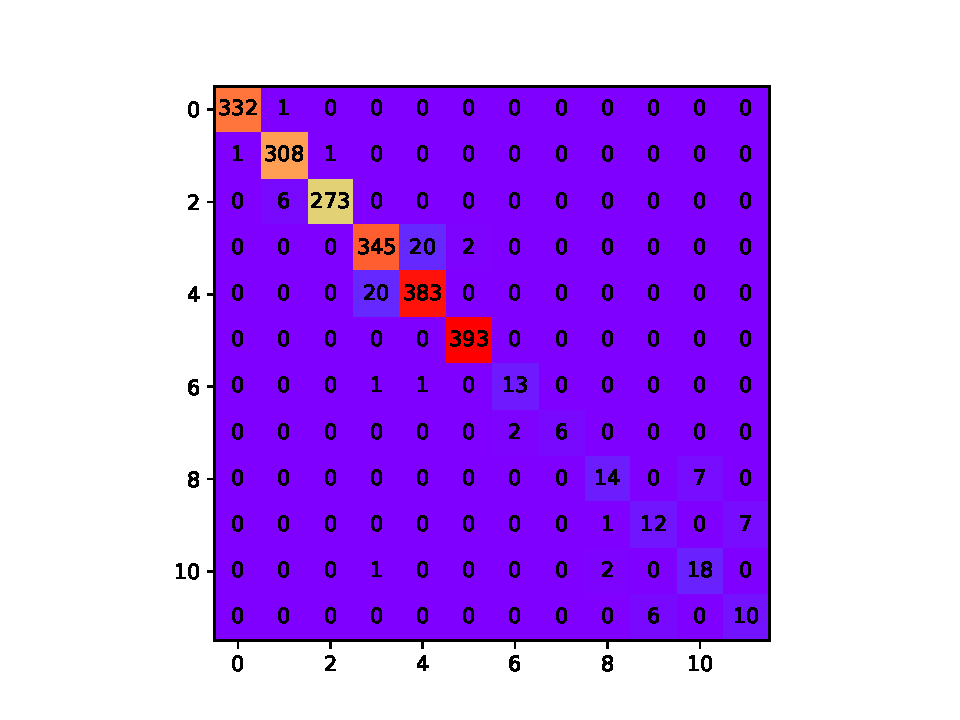
\includegraphics[scale=0.45]{matrix_svm.pdf}}
	\subfigure[Matriz de Confusão - Perceptron]{
		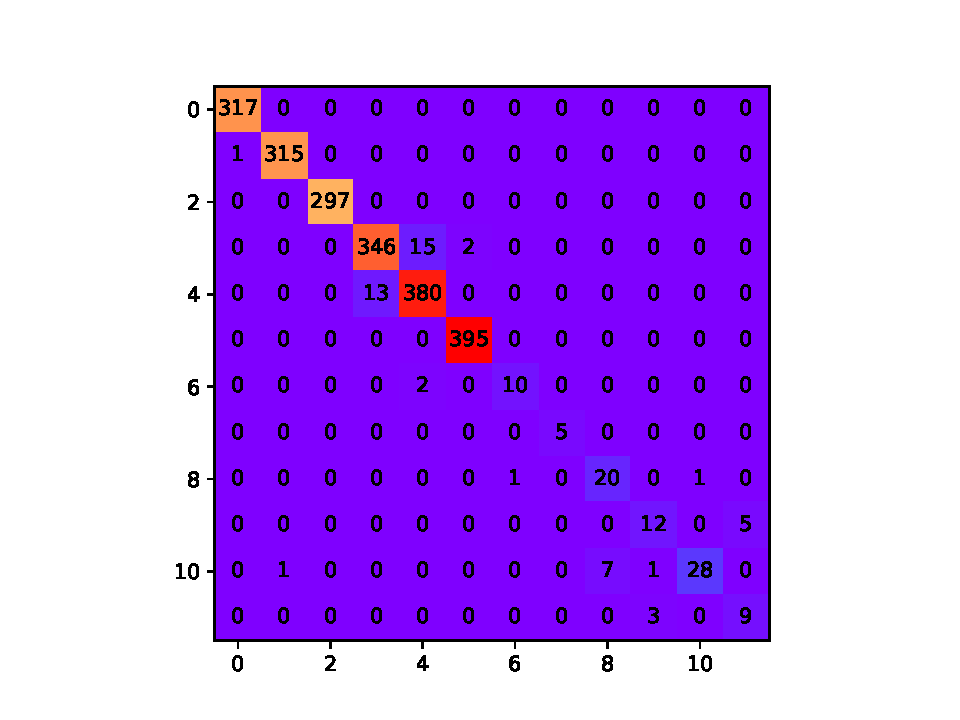
\includegraphics[scale=0.45]{matrix_perceptron.pdf}}
	\caption{Comparação entre Matrizes de confusão}
	\label{fig:confusao}
	\end{figure}




\newpage

\section{Conclusões}
	Este trabalho permitiu a compreensão de alguns métodos de aprendizagem. A escolha de cada método deve ser adequada ao tipo dos dados a serem aprendidos e, neste caso, a não uniformidade da quantidade de informações sobre cada característica gerou uma diferença consideral entre cada método. Também notou-se que a técnica PCA não necessariamente colabora com os resultados, por exemplo, no método Perceptron, quanto mais características, melhor foram os resultados. Outro fator notável, foi o ganho ao aumentar a quantidade de classes, isso gerou um ganho relativamente pequeno de acurácia e aumentou o tempo de computação consideravelmente. De forma conclusiva, não houve um método com destaque nos resultados obtidos, as diferenças foram sutis e todos foram considerados satisfatórios.

\bibliographystyle{sbc}
\bibliography{sbc-template}

\end{document}
